\noindent The world is filled with a great variety of objects, yet people have little difficulty making sense of them. 
Presented with a novel object, people can readily identify its parts \shortcite{schyns1994ontogeny}, guess its function \shortcite{tversky1984objects}, and refer to it unambiguously \shortcite{hawkins2020characterizing}. 
These abilities rest on the capacity to robustly connect features of the external world to a rich library of mental concepts describing not just whole objects, but their parts and how they are arranged \shortcite{miller2013language, landau1993and, rosch1975family,mukherjee2019communicating}. 

For example, consider the bottom-most \emph{gadget} in Fig.~\ref{fig:task}A: even though this object does not correspond to a familiar category, we may say that it contains a row of \texttt{buttons} or \texttt{dials}, and that it is topped by an \texttt{antenna} or a \texttt{knob}.
But just as we do not have a pre-existing concept for every object we encounter, we do not have a concept corresponding to every part: in Fig.~\ref{fig:task}A, for example, most people do not have a concept corresponding to a \texttt{row of exactly five dials}. %, or a \texttt{box with an antenna on top}. 
Indeed, a complex object can be decomposed in combinatorially many ways, but people are likely to favor only a tiny subset of these.
What characterizes the set of part concepts that people do use? Why these, and not others?
%Indeed, a complex object can be decomposed into combinatorially many substructures like these, but a typical human will analyze an object using only a tiny subset of these. What characterizes the set of concepts that humans \emph{do} have? Why these, and not others?
% \jda{someone fill in: what is a concept, and what does it mean to ``have'' a concept}

% how do we connect inputs to percepts/concepts
% Moreover, a core challenge is to explain why certain ways of carving up the visual world are more compelling 
Identifying which parts people use to parse the visual world has been a core goal for classic theories of perceptual organization \shortcite{palmer1977hierarchical,marr1978representation,hoffman1984parts,biederman1987recognition,hummel1992dynamic} and continues to pose challenges for modern vision models \shortcite{mo2019partnet, bear2020learning, hinton2021represent}.
But how can we tell whether any of these proposals actually explain visual object understanding? 
Empirical tests of these theories have generally relied upon simple discrimination tasks rather than richer behavioral readouts, limiting their ability to evaluate correspondences between a candidate representation of a given object and the full set of parts and relations that people can identify.

% \todo[inline]{moreover, we'd like to go beyond identification to begin to explain \emph{why} these particular parts and not some other set of parts. i.e. emerge from rational analysis.}
% how do we connect from percepts to linguistically expressible concepts?
% Meanwhile, it is not obvious which level of abstraction  relevant for characterizing its structure.
% How do people actually decompose these objects when describing their structure? And what are the principles that explain why they decompose them one way instead of another?
% There is considerable evidence that languages have been shaped by communicative need to expose relevant structure in the world \shortcite{rosch1976basic, tversky1984objects}. 
% We do not have words for every possible part decomposition, hence the parts that do become lexicalized in our vocabulary may be the product of resolving a tradeoff between informativeness and cognitive economy \shortcite{regier201511,kirby2015compression,zaslavsky2018efficient}.
% This paper seeks to answer both questions. 
% To do so, 

% \jda{someone fill this in: not \jda {exactly the regier et al cites, but instead support for the claim ``has a lexicon entry'' = ``has a concept''}. 
% Both components of this approach have a long history in cognitive science: 
% \jda{still missing some cites here}
%%%%%%
% \jda{what's new about our synthesis of these tools? relative to the efficient comm literature, something like ``we're not just studying words, but the internal structure of the concepts they specify''}
%%%%%%

Here, we leverage \textit{language} to identify the concept library used for visual object understanding, and \textit{programs} to capture how object parts and relations are internally represented (Fig.~\ref{fig:task}B).
% Here we leverage \emph{language} as a source of evidence for the human concept library, and \emph{programs} as representations of the internal structure of concepts.
Natural language production tasks are an especially powerful tool towards this end, given abundant evidence that our vocabularies have been shaped to efficiently communicate about the concepts we find relevant \shortcite{regier201511,kirby2015compression,zaslavsky2018efficient,sun2021seeing}.

In Part I, we describe our strategy for synthesizing a diverse collection of novel objects and eliciting open-ended descriptions from people about their structure.
Analyzing these descriptions reveals a distinctive feature of the concept library: individual part concepts are not arbitrarily complex, and as objects increase in complexity, their descriptions become longer rather than reliant on more complex concepts.
In Part II, we refine this picture of the concept library by formalizing concept identification as search over a space of graphics libraries that vary in the visual part concepts they contain, building on recent work in program library discovery \shortcite{ellis2020dreamcoder,tian2020learning, wang2021learning,wong2021leveraging}.
We discover that a preference for part concepts of intermediate complexity is not arbitrary, but reflects a fundamental trade-off between the complexity of the concept library and the complexity of objects represented using that library. 
In sum, our findings highlight the value of jointly leveraging program representations and naturalistic language at scale to expose the internal structure of the object and part concepts we use to make sense of the world. 

% We show that a preference for bounded concept complexity is not arbitrary, but instead reflects a fundamental trade-off between the complexity of the library and the complexity of individual object analyses. We show that human lexical choice is best explained by libraries that \emph{optimize a description length criterion}: minimizing the total number of concepts in the library plus the length of an average stimulus expressed in terms of those concepts.
% We show that human lexical choice is best explained by libraries that \emph{optimize a description length criterion}: minimizing the length of all the programs in the library plus the length of an average stimulus expressed in terms of those programs.

% To explore this possibility, here we leverage the language people use to describe a large and varied set of novel objects to uncover the part concepts that people deem most relevant for characterizing their structure.
% We formalize our problem as search over the space of graphics libraries that vary in the visual part concepts they contain, building on recent work in program library discovery \shortcite{ellis2020dreamcoder,tian2020learning, wang2021learning}.
% We then evaluate how well the programs written in each library predict how much and what people say (Fig.~\ref{fig:task}B).
% % explain quantitative and qualitative patterns in human language.
% While a ``base'' library containing only the simplest shape primitives (e.g., block) explains some variance in the length of linguistic descriptions, we found that libraries containing moderately complex part concepts (e.g., pillar) provide both efficient compression of these objects and better explain the way people describe them.

% In \textbf{Part I}, we describe a procedure for generating complex but naturalistic visual stimuli that can be described by programs. Using this procedure, we collect a large dataset of images paired with both programmatic and natural language descriptions. Analyzing these descriptions reveals a distinctive feature of the concept library: individual concepts are \emph{boundedly complex}, and as stimuli grow more complex, their descriptions become \emph{longer} rather than reliant on more complex concepts.
% In \textbf{Part II}, we refine this picture of the concept library. We show that a preference for bounded concept complexity is not arbitrary, but instead reflects a fundamental trade-off between the complexity of the library and the complexity of individual object analyses. We show that human lexical choice is best explained by libraries that \emph{optimize a description length criterion}: minimizing the total number of concepts in the library plus the length of an average stimulus expressed in terms of those concepts.
% % We show that human lexical choice is best explained by libraries that \emph{optimize a description length criterion}: minimizing the length of all the programs in the library plus the length of an average stimulus expressed in terms of those programs.
% Together, these results suggest that the human concept inventory, like \jda{someone fill in: various other aspects of human cognition}, reflects a sophisticated trade-off between complexity and explanatory adequacy, and that the internal structure of concepts (modeled as programs and revealed in lexical choice) is an important component of this trade-off.
%%%%%%
% \jda{This is also a place we could distinguish what we're doing from noga/terry r/ted g-type work}
%%%%%

\begin{comment}

%%%% PHENOMENON: How do we talk about structure in the world? 
\noindent The world is filled with a great variety of objects, yet people have no trouble finding ways to talk about them. 
People not only know what to call a given object, but also how to describe its structure --- what parts it is composed from and how those parts are arranged.
% In other words, the underlying structure of our percepts and concepts is often reflected in the structure of our language \cite{miller2013language,landau1993and}.
In other words, our experience of structure in the visual world and the language we use to communicate about it appear to be closely coupled \cite{miller2013language,landau1993and}.
For example, a car has a \emph{body}, \emph{windows}, \emph{doors}, and \emph{wheels}.
Houses also have \emph{doors} and \emph{windows} (even if they look different from those of cars), but may be multiple \emph{stories} and have a \emph{roof} on top.
Even for an object someone has never seen before, people can generally figure out how to describe it so that they are understood \cite{hawkins2020characterizing}. 
What does the way we talk about objects reveal about how their structure is represented in the mind?

% What  enable people to so robustly communicate their understanding of how objects are organized?

%%%% PERCEPTION
Uncovering the perceptual units by which people parse the visual world has been a core target for classic theories of perception \shortcite{palmer1977hierarchical,marr1978representation,hoffman1984parts,hummel1992dynamic} and continues to pose challenges for modern vision models \shortcite{mo2019partnet, bear2020learning, hinton2021represent}.
Proposed solutions have varied widely, from defining a fixed set of volumetric primitives \shortcite{biederman1987recognition}, to using dimensionality reduction \shortcite{lee1999learning} or probabilistic inference \shortcite{austerweil2013nonparametric} to recover a part basis over image-like representations.
However, empirical tests of these proposals have largely been limited to simple discrimination or judgment tasks, limiting their ability to evaluate detailed correspondences between each putative representation and the full set of parts and relations that people can identify.
% making it challenging to evaluate the precise abstractions being used at an instance-by-instance level. 

%%%% LANGUAGE
Natural language behavior may provide a promising alternative way to access these representations. 
For example, consider the drawings in the left column of Fig. \ref{fig:task}A.
Someone could fully describe each drawing in terms of a few basic shapes (e.g., \textit{lines, circles}), by using names for larger units (e.g., \textit{dial}, \textit{drawer}), or even by producing a single phrase that refers to multiple parts.
How do people actually decompose these objects when describing their structure? And what are the principles that explain why they decompose them one way instead of another?
There is considerable evidence that languages have been shaped by communicative need to expose relevant structure in the world \shortcite{rosch1976basic, tversky1984objects}. 
We do not have words for every possible part decomposition, hence the parts that do become lexicalized in our vocabulary may be the product of resolving a tradeoff between informativeness and cognitive economy \shortcite{regier201511,kirby2015compression,zaslavsky2018efficient}.
% Meanwhile, many other visual motifs are more costly to express in words.

To explore this possibility, here we leverage the language people use to describe a large and varied set of novel objects to uncover the part concepts that people deem most relevant for characterizing their structure.
We formalize our problem as search over the space of graphics libraries that vary in the visual part concepts they contain, building on recent work in program library discovery \shortcite{ellis2020dreamcoder,tian2020learning, wang2021learning}.
We then evaluate how well the programs written in each library predict how much and what people say (Fig.~\ref{fig:task}B).
% explain quantitative and qualitative patterns in human language.
While a ``base'' library containing only the simplest shape primitives (e.g., block) explains some variance in the length of linguistic descriptions, we found that libraries containing moderately complex part concepts (e.g., pillar) provide both efficient compression of these objects and better explain the way people describe them.

\end{comment}
% Taken together, our findings highlight the value of measuring naturalistic language behavior at scale and using structured program representations for exposing the perceptual units that organize our understanding of the visual world.

% In this paper, we propose a new approach for probing conceptual structure through linguistic descriptions.
% In particular, we build on the recent proposal that object concepts may be represented as graphics \textit{programs} written in a domain-specific language (DSLs) defined over a \emph{library} of compositional primitives \shortcite{goodman2014concepts,lake2015human,ellis2020dreamcoder,tian2020learning}, each corresponding to a meaningful part.
% We begin by examining a large corpus of procedural descriptions for a variety of complex objects (Part I). 
% Then, by predicting participants' descriptions from programs expressed in different DSLs (Part II), we begin to identify the levels of conceptual abstraction that best explain behavior.

%, building on classic notions of a compositional mental language of thought. 
%Yet, for all of these proposals, it has been challenging to predict exactly how people will decompose a given object. 
%Classic work was limited to eliciting relatively low-bandwidth judgments and recent work has focused on relatively simple scenes.
% What determines the basic level of abstraction a person chooses to describe these compositional stimuli, amongst the possible vocabularies of nameable parts?

%%%% PROGRAM-LIKE CONCEPTS
% We approach this question through a formal computational model that builds on two related lines of work. Prior word learning models \shortcite{xu2007word,frank2009using} have proposed that for \textit{individual} category names, contextual word choice can be modeled as Bayesian optimality over a hypothesis space of alternatives. Agents may build on an initial library of primitive concepts with new \textit{abstractions}, chunked subroutines which abstract over programs written in lower-level primitives. Prior experimental work has used models of program \textit{abstraction} learning to explain people's motor abstraction learning over domains of compositional drawing stimuli \shortcite{tian2020learning}; and to model human coordination on shared object representations when assembling simple, compositional block towers \shortcite{mccarthy2021learning}.


%%%% FRAMEWORK TO INFER CONCEPT LIBRARY PEOPLE USING TO COMMUNICATE ABOUT OBJECT STRUCTURE
\begin{figure*}[ht!]
  \begin{center}
  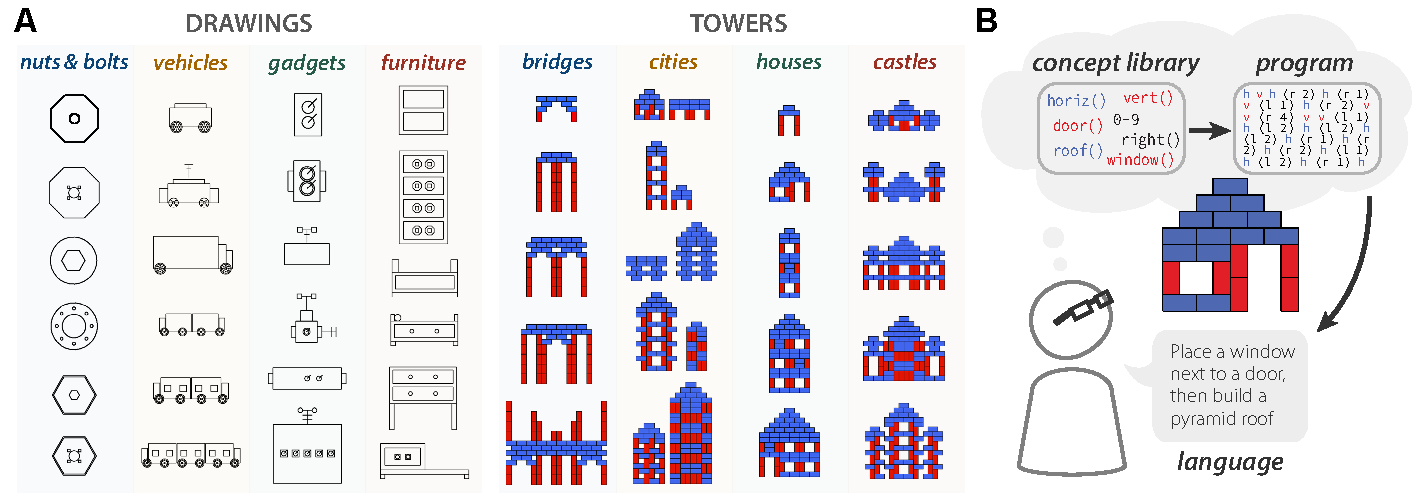
\includegraphics[width=1.02\linewidth]{figures/lax_task.pdf}
  \caption{(A) Example objects from the \textit{Drawings} and \textit{Towers} domains. Each domain contains 4 subdomains of 250 novel objects. Each domain and subdomain was designed to include high variation over the type and number of base primitives (i.e., shapes, blocks). (B) This work aims to infer the latent concept library that people are using to decompose complex objects into parts, where objects are represented by executable graphics programs.}
  \label{fig:task}
  \end{center}
 \end{figure*}



% In this paper,  we suggest that the \textit{level of abstraction} people choose when describing a domain of compositional objects -- like the \textit{technical drawings} and \textit{block towers} in Fig. \ref{fig:task}A -- can be modeled as a \textit{DSL choice} over possible libraries of formal conceptual primitives at differing levels of abstraction, which can be composed into generative programs to produce any chosen object. We hypothesize that the level of abstraction reflects a contextual tradeoff between \textbf{DSL size} (the total number of concepts necessary to represent objects in a given domain, using a particular set of conceptual primitives) and \textbf{program description length} (how many primitives in the chosen DSL must be composed to describe any individual item drawn from the domain). This hypothesis formalizes an intuitive tradeoff in classical, part-based theories of the basic level: a low-level set of parts (like describing the drawing in terms of \textit{squares} and \textit{circles}) uses a small vocabulary, but requires  many words to describe an individual object; a high-level but specific set of parts (one with specialized terms for different makes and models of dressers, for instance) might succinctly describe any one object, but at the expense of requiring a large overall vocabulary to describe a diverse domain.

% To evaluate this, we develop a dataset of two domains of hierarchical object stimuli (Fig. \ref{fig:task}A), and conduct a procedural language experiment to elicit human descriptions of each object. We find that people use different, context-specific linguistic vocabularies dependent on the subdomain of objects (Part I). We then introduce the formal representational approach, defining program \textit{DSLs} at varying levels of abstraction, that we use to model abstraction choice in language. Using this, we first use \textit{program description length} alone to correlate programs and language (Part II), and discuss findings and challenges of this approach. Finally, we introduce a more expressive \textit{program-language alignment} model, and find that people's language is best explained in this model by DSLs that jointly minimize program description length \textit{and} overall DSL size (Part III).